\chapter{Bivariantna analiza}

\section{T-test}

\subsection{T-test za (parne) odvisne vzorce}

Primerjava povprečij dveh pogojev, v katerih so sodelovale iste enote.

Primer: 20 študentov je dobilo test v izpolnjevanje pred študijem določenega predmeta in nato ponovno po zaključku tega predmeta.

Testna statistika $t=\frac{\bar{d}}{SE(\bar{d})}$.

Izračun:

\begin{enumerate}
    \item Postavimo ničelno in alternativno hipotezo:
        \begin{itemize}
            \item $H_0$: Ni razlik v znanju študentov pred in po študiju tega modula.
            \item $H_1$: Obstajajo razlike v znanju študentov pred in po študiju tega modula.
        \end{itemize}
    \item Izračunamo razlike med pari opazovanj: $d_i = y_i - x_i$ (za vajo lahko to naredimo v SPSS).
    \item Izračunamo povprečje razlik: $\bar{d}$.
    \item Standardni odklon razlik: $s_d$.
    \item Standardna napaka povprečne razlike: $SE(\bar{d}) = \frac{s_d}{\sqrt{n}}$.
    \item T-statistika: $t = \frac{\bar{d}}{SE(\bar{d})}$ (empirična vrednost); $df = n-1$.
    \item V tabeli poiščemo kritično vrednost pri $\alpha = 5\%$.
    \item Empirična vrednost $t$ pade v kritično območje, ki ga določa teoretična vrednost $t$ pri dani stopnji zaupanja, zato lahko zavrnemo ničelno hipotezo in sprejmemo alternativno. Napiši kaj, če ne pade v kritično območje!
    \item Interval zaupanja za resnično vrednost razlike povprečij je: 
        \[\bar{d} \pm (t \cdot SE(\bar{d}))\]
\end{enumerate}

\subsection{T-test za neodvisne vzorce}

Primerjava preizkusa domneve o srednjih vrednosti dveh skupin enot.

Primer: Primerjava kalorične vrednosti dveh vrst štrudlja.

Testna statistika $t = \frac{\bar{x_1}-\bar{x_2}}{SE(\bar{x_1}-\bar{x_2})}$.

Opomba: Test predpostavi enakost varianc neodvisnih vzorcev. Če to ni zagotovoljeno, uporabimo Welchov test $t = \frac{\bar{x_1}-\bar{x_2}}{\sqrt{\frac{s_1^2}{n_1}+\frac{s_2^2}{n_2}}}$.

Izračun:
\begin{enumerate}
    \item Postavimo ničelno in alternativno hipotezo:
        \begin{itemize}
            \item $H_0$: Ni razlik v kalorični vsebnosti med dvema vrstama hotdoga.
            \item $H_1$: So razlike v kalorični vsebnosti med dvema vrstama hotdoga.
        \end{itemize}
    \item Razlika med povprečnima vrednostima: $\bar{x}_1 - \bar{x}_2$.
    \item Skupni standardni odklon (pod predpostavko enakih varianc):
        \[s_p = \sqrt{\frac{(n_1 - 1) \cdot s_1^2 + (n_2 - 1) \cdot s_2^2}{n_1 + n_2 - 2}}\]
    \item Standardna napaka: 
        \[SE(\bar{x}_1 - \bar{x}_2) = s_p \cdot \sqrt{\frac{1}{n_1} + \frac{1}{n_2}}\]
    \item Empirična t-vrednost: 
        \[t = \frac{\bar{x}_1 - \bar{x}_2}{SE(\bar{x}_1 - \bar{x}_2)}\]
    \item Prostostne stopnje: $df = n_1 + n_2 - 2$.
    \item V tabeli poiščemo kritično vrednost pri $\alpha = 5\%$.
    \item Interval zaupanja za resnično vrednost razlike povprečij: 
        \[\bar{x}_1 - \bar{x}_2 \pm (t \cdot SE(\bar{x}_1 - \bar{x}_2))\]
\end{enumerate}

\section{Analiza variance (ANOVA)}

Primerjava povprečij večih skupin (če sta samo dve skupini, je ANOVA enaka T testu).

$F$ porazdelitev ima dve prostorski skopnji.

\begin{figure}[h]
    \centering
    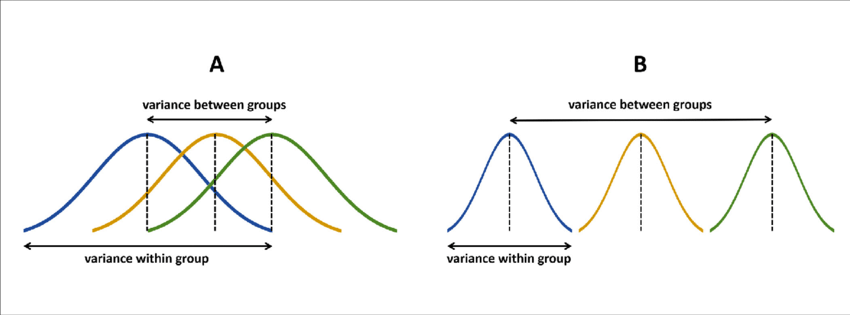
\includegraphics[width=\textwidth]{pictures/anova_varianca.png}
    \caption{This is a caption for the figure.}
    \label{fig:anova_varianca}
\end{figure}

Primer: Tri skupine desetih slučajno izbranih študentov so postavljene v tri različne učilnice. A ima konstantno glasbo v ozadju, B variabilno glasbo v ozadju, C brez glasbe. Po enem mesecu nas zanima, ali glasba pomaga pri učenju.

Izračun:
\begin{enumerate}
    \item Postavimo ničelno in alternativno hipotezo:
        \begin{itemize}
            \item $H_0$: Med skupinami ni razlik v vsrkavanju informacij.
            \item $H_1$: Med skupinami so razlike v vsrkavanju informacij.
        \end{itemize}
    \item Izračunamo povprečja. Skupno povprečje je $\bar{x} = 5,1$, povprečja posameznih skupin pa so $\bar{x}_1 = 7$, $\bar{x}_2 = 4$, in $\bar{x}_3 = 4,3$.
    \item Vsota kvadratov:
        \begin{itemize}
            \item Med skupinami: $SS_{between} = 54,6$
            \item Znotraj skupin: $SS_{within} = 90,1$
        \end{itemize}
    \item Prostostne stopnje:
        \begin{itemize}
            \item Med skupinami: $df_{between} = 2$
            \item Znotraj skupin: $df_{within} = 27$
        \end{itemize}
    \item Povprečni kvadrat:
        \begin{itemize}
            \item Med skupinami: $MS_{between} = \frac{SS_{between}}{df_{between}} = \frac{54,6}{2} = 27,3$
            \item Znotraj skupin: $MS_{within} = \frac{SS_{within}}{df_{within}} = \frac{90,1}{27} = 3,34$
        \end{itemize}
    \item Empirična F-vrednost: 
        \[F = \frac{MS_{between}}{MS_{within}} = \frac{27,3}{3,34} = 8,18\]
    \item V tabeli poiščemo kritično vrednost pri $\alpha = 5\%$: $F_{critical} = 2,03$.
    \item Ker je empirična F-vrednost (8,18) večja od kritične vrednosti (2,03), zavrnemo ničelno hipotezo $H_0$.
    \item Izračunamo eta kvadrat ($\eta^2$), ki je merilo učinka:
        \[\eta^2 = \frac{SS_{between}}{SS_{between} + SS_{within}} = \frac{54,6}{54,6 + 90,1} = 0,38\]
        \[ \eta = \sqrt{\eta^2} = \sqrt{0,38} \approx 0,62\]
\end{enumerate}

\section{Neparametrične alternative}

Če podatki niso normalno porazdeljeni, moramo parametrični test zamenjati z ustreznim neparametričnim testom.

\begin{table}[h!]
    \centering
    \begin{tabular}{|l|l|l|}
    \hline
    \textbf{Cilj} & \textbf{Parametrični test} & \textbf{Neparametrični test} \\ \hline
    Testiranje razlike med dvema odvisnima nizoma enot & Odvisni $t$-test & Wilcoxon test predznačenih rangov \\ \hline
    Testiranje razlike med dvema neodvisnima nizoma enot & Neodvisni $t$-test & Mann-Whitney $U$ test \\ \hline
    Testiranje razlike med tremi ali več neodvisnimi nizi enot & ANOVA & Kruskal-Wallis $H$ test \\ \hline
    \end{tabular}
    \caption{Pregled parametričnih in neparametričnih testov}
\end{table}

\subsection{Hi-kvadrat test}

Uporablja se za ugotavljanje, ali obstaja statistično značilna razlika med pričakovanimi in opazovanimi frekvencami v eni ali več kategorijah (torej če imamo nomilane spremenljivke)

Ničelna hipoteza $H_0$: V populaciji ni povezanosti med spremenljivkama.

Slika hi kvadrat porazdelitve

\paragraph{Izračunavanje stopnje prostosti ($df$):}
Stopnja prostosti ($df$) za hi-kvadrat test se izračuna po formuli:
\[df = (\text{vrstice} - 1) \cdot (\text{stolpci} - 1)\]

\paragraph{Postopek izračuna:}
\begin{enumerate}
    \item Zberemo podatke in uredimo frekvence v kontingenčni tabeli.
    \item Izračunamo pričakovane frekvence za vsako celico tabele.
    \item Uporabimo formulo za hi-kvadrat vrednost:
    \[\chi^2 = \sum \frac{(O_i - E_i)^2}{E_i}\]
    kjer je $O_i$ opazovana frekvenca, $E_i$ pa pričakovana frekvenca.
\end{enumerate}

\paragraph{Uporaba kontingenčnih koeficientov:}
Ker vrednosti hi-kvadrat same po sebi niso primerljive med različnimi tabelami, pogosto uporabimo kontingenčne koeficiente, kot je Cramérjev $V$, ki ga izračunamo po formuli:
\[V = \sqrt{\frac{\chi^2}{N \cdot (k - 1)}},\]
kjer je $\chi^2$ hi-kvadrat vrednost, $N$ skupno število opazovanj, $k$ pa število kategorij v najbolj številni spremenljivki.

\subsection{Spearmanov koeficient}

Spearmanov koeficient korelacije meri moč in smer monotone povezave med dvema spremenljivkama. Uporablja se za ordinalne spremenljivke ali za kvantitativne spremenljivke, ki niso nujno normalno porazdeljene.

\paragraph{Ničelna hipoteza $H_0$:}
Med dvema spremenljivkama ni monotone povezave.

\paragraph{Formula:}
Spearmanov koeficient ($\rho$) se izračuna po formuli:
\[\rho = 1 - \frac{6 \sum d_i^2}{n(n^2 - 1)},\]
kjer je $d_i$ razlika med vrstnimi številkami vsakega opazovanja in $n$ število opazovanj.

\paragraph{Postopek izračuna:}
\begin{enumerate}
    \item Razvrstimo podatke v naraščajočem vrstnem redu za vsako spremenljivko.
    \item Izračunamo vrstne številke za vsako spremenljivko.
    \item Izračunamo razlike med vrstnimi številkami ($d_i$) za vsako opazovanje.
    \item Uporabimo zgornjo formulo za izračun Spearmanovega koeficienta.
\end{enumerate}

\paragraph{Interpretacija:}
Spearmanov koeficient se giblje med -1 in 1. Vrednost blizu 1 kaže na močno pozitivno monotono povezavo, vrednost blizu -1 kaže na močno negativno monotono povezavo, vrednost blizu 0 pa kaže na odsotnost monotone povezave.

\paragraph{Zaključek:}
Spearmanov koeficient je uporaben za analizo povezav med ordinalnimi ali kvantitativnimi spremenljivkami, ki niso normalno porazdeljene. Pomaga nam razumeti moč in smer monotone povezave med spremenljivkami.

\subsection{Pearsonov koeficient}

Pearsonov koeficient korelacije meri linearno povezanost med dvema kvantitativnima spremenljivkama. Uporablja se za intervalne ali razmerne spremenljivke, ki so normalno porazdeljene.

\paragraph{Ničelna hipoteza $H_0$:}
Med dvema spremenljivkama ni linearne povezave.

\paragraph{Formula:}
Pearsonov koeficient ($r$) se izračuna po formuli:
\[r = \frac{\sum (x_i - \bar{x})(y_i - \bar{y})}{\sqrt{\sum (x_i - \bar{x})^2 \sum (y_i - \bar{y})^2}},\]
kjer je $x_i$ in $y_i$ vsaka opazovanja za spremenljivki $x$ in $y$, $\bar{x}$ in $\bar{y}$ pa povprečji za spremenljivki $x$ in $y$.

\paragraph{Postopek izračuna:}
\begin{enumerate}
    \item Izračunamo povprečje za vsako spremenljivko.
    \item Izračunamo odstopanja vsakega opazovanja od povprečja.
    \item Pomnožimo odstopanja za ustrezna opazovanja in izračunamo vsoto.
    \item Izračunamo kvadrate odstopanj za vsako spremenljivko in vsoto kvadratov.
    \item Uporabimo zgornjo formulo za izračun Pearsonovega koeficienta.
\end{enumerate}

\paragraph{Interpretacija:}
Pearsonov koeficient se giblje med -1 in 1. Vrednost blizu 1 kaže na močno pozitivno linearno povezavo, vrednost blizu -1 kaže na močno negativno linearno povezavo, vrednost blizu 0 pa kaže na odsotnost linearne povezave.

\section{Povezanost}

Povezanost med dvema spremenljivkama pomeni, da spremembe v eni spremenljivki sovpadajo s spremembami v drugi spremenljivki. Povezanost lahko merimo na različne načine, odvisno od narave spremenljivk in vrste povezave.

\subsection*{Funkcionalna povezanost}
Funkcionalna povezanost pomeni, da obstaja točno določena matematična funkcija, ki povezuje dve spremenljivki. Na primer, če $y = f(x)$, potem je $y$ popolnoma določeno s $x$. To je najmočnejša oblika povezanosti, saj vsaka vrednost ene spremenljivke določa točno eno vrednost druge spremenljivke.

\subsection*{Korelacijska povezanost}
Korelacijska povezanost meri stopnjo in smer linearne povezave med dvema kvantitativnima spremenljivkama. Najpogosteje uporabljamo Pearsonov koeficient korelacije ($r$), ki meri linearno povezanost, in Spearmanov koeficient korelacije ($\rho$), ki meri monotono povezanost.

\subsection*{Močna in šibka povezanost}
Moč povezanosti se nanaša na velikost koeficienta korelacije. 
\begin{itemize}
    \item \textbf{Močna povezanost}: Koeficient korelacije blizu 1 ali -1 kaže na močno povezanost.
    \item \textbf{Šibka povezanost}: Koeficient korelacije blizu 0 kaže na šibko povezanost.
\end{itemize}

\subsection*{Linearna in nelinearna povezanost}
\begin{itemize}
    \item \textbf{Linearna povezanost}: Povezanost, kjer lahko povezavo med spremenljivkama najbolje opišemo z ravno črto. Pearsonov koeficient korelacije ($r$) je primeren za merjenje linearne povezanosti.
    \item \textbf{Nelinearna povezanost}: Povezanost, kjer je povezava med spremenljivkama bolj zapletena in je ni mogoče opisati z ravno črto. Spearmanov koeficient korelacije ($\rho$) je primeren za merjenje monotone (nelinearne) povezanosti.
\end{itemize}

\subsection*{Pozitivna in negativna povezanost}
\begin{itemize}
    \item \textbf{Pozitivna povezanost}: Ko se ena spremenljivka povečuje, se druga spremenljivka tudi povečuje. Koeficient korelacije je pozitiven.
    \item \textbf{Negativna povezanost}: Ko se ena spremenljivka povečuje, se druga spremenljivka zmanjšuje. Koeficient korelacije je negativen.
\end{itemize}

\subsection{Kovarianca}

Kovarianca je mera, ki opisuje, kako se dve spremenljivki sočasno spreminjata. Pozitivna kovarianca pomeni, da se večje vrednosti ene spremenljivke povezujejo z večjimi vrednostmi druge spremenljivke, medtem ko negativna kovarianca pomeni, da se večje vrednosti ene spremenljivke povezujejo z manjšimi vrednostmi druge spremenljivke.

\paragraph{Formula}
Kovarianca dveh spremenljivk $X$ in $Y$ se izračuna po formuli:
\[\text{Cov}(X, Y) = \frac{1}{n-1} \sum_{i=1}^n (X_i - \bar{X})(Y_i - \bar{Y}),\]
kjer:
\begin{itemize}
    \item $X_i$ in $Y_i$ sta posamezni opazovanji spremenljivk $X$ in $Y$,
    \item $\bar{X}$ in $\bar{Y}$ sta povprečji spremenljivk $X$ in $Y$,
    \item $n$ je število opazovanj.
\end{itemize}

\paragraph{Interpretacija}
\begin{itemize}
    \item \textbf{Pozitivna kovarianca}: Ko se vrednosti ene spremenljivke povečujejo, se povečujejo tudi vrednosti druge spremenljivke.
    \item \textbf{Negativna kovarianca}: Ko se vrednosti ene spremenljivke povečujejo, se vrednosti druge spremenljivke zmanjšujejo.
    \item \textbf{Kovarianca blizu nič}: Ni jasno izražene povezave med spremenljivkama.
\end{itemize}

\paragraph{Razlika med kovarianco in korelacijo}

Kovarianca meri le smer sočasnih sprememb dveh spremenljivk, vendar ni standardizirana, zato njena vrednost ni omejena. Po drugi strani pa je korelacija standardizirana mera, ki pove, kako močna in v katero smer je linearna povezava med dvema spremenljivkama, njena vrednost pa je vedno med -1 in 1.

\begin{Vaje}{1}
    V datoteki \href{https://github.com/borbregant/ai_tandem_learning/blob/main/data_cleaned.xlsx}{data\_cleaned.xlsx} določi naslednje:
    \begin{itemize}
        \item Ali obstaja povezava med matematično anksioznostjo in motivacijo za matematiko? Če je povezava znatna, določi še enačbo linearne regresije, kjer si sam izbereš odvisno in neodvisno spremenljivko.
        \item Ali obstaja povezava med spolom in anksioznostjo?
        \item Ali obstaja povezava med profesorjem in razredom?
    \end{itemize}
    Imej v mislih, da so kategorične spremenljivke v dokumentu kodirane označevalno.
\end{Vaje}
